\documentclass[9pt]{beamer}

\usepackage{hyperref}
\usepackage[utf8]{inputenc} 
\usepackage[english]{babel}
\usepackage{fancyhdr}
\usepackage{amsmath,amssymb}
\usepackage{array}
%\usepackage{style}
\usepackage{amsthm}
\usepackage[toc,page]{appendix}
\usepackage{color}
\usepackage{graphicx}
\usepackage{frontespizio}
\usepackage{faktor}
\usepackage{hyperref}
\usepackage{frontespizio}
\usepackage{pdfpages}
\usepackage{listings}
\usepackage{import}
\usetheme{JuanLesPins}
\usefonttheme{serif}
\newcommand{\sg} {
  \boldsymbol{\mu}}
 \newcommand{\Nd}{N_{\delta}}
\newcommand{\Nc}{N}
\newcommand{\Bc}{\mathcal{B}}
\newcommand{\bu}{\textbf{u}}
\newcommand{\bv}{\textbf{v}}
\usepackage{verbatim}
\usepackage{afterpage}
\newcommand{\og}{\omega}


\title{Imbalanced Binary Classification}
\author{Julien Genovese}
\institute{Machine Learning Together Milan}
\date{January 2021}

\AtBeginSection[]{
  \begin{frame}
  \vfill
  \centering
  \begin{beamercolorbox}[sep=8pt,center,shadow=true,rounded=true]{title}
    \usebeamerfont{title}\insertsectionhead\par%
  \end{beamercolorbox}
  \vfill
  \end{frame}
}
\AtBeginSubsection[]{
  \begin{frame}
  \vfill
  \centering
  \begin{beamercolorbox}[sep=8pt,center,shadow=true,rounded=true]{title}
    \usebeamerfont{title}\insertsubsectionhead\par%
  \end{beamercolorbox}
  \vfill
  \end{frame}
}

\setbeamertemplate{bibliography item}{\insertbiblabel}
\usepackage{filecontents}
\begin{filecontents}{abc.bib}
@book{apm,
title={Applied Predictive Modeling},
author={Max Kuhn, Kjell Johnson},
journal={Springer},
pages={419--443},
year={2016}
}
\end{filecontents}


\begin{document}


\begin{frame}
\maketitle
\begin{figure}[ht]

\includegraphics[scale=0.25]{images/MLTM.jpeg}
\quad
\end{figure}
\end{frame}

\begin{frame}
\frametitle{Table of Contents}
\tableofcontents
\end{frame}
\section{Introduction to imbalanced binary problems}
\begin{frame}
\frametitle{Definition of imbalanced binary classification problem}
\begin{itemize}
\item It's a \textbf{binary classification problem} where the target output is composed by \textbf{two classes where one of them is more frequent than the other one}. 
\vspace{3mm}
\begin{figure}[ht]
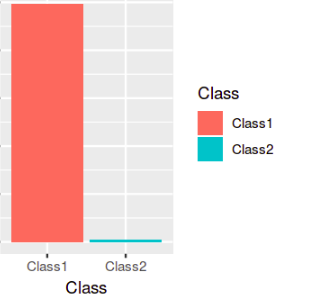
\includegraphics[scale=0.50]{images/imbalance.png}
\caption{A classical example of imbalance}
\end{figure}
\item A \textbf{very common problem} in real datasets. 
\end{itemize}
\end{frame}

\begin{frame}
\frametitle{Two examples}
\begin{itemize}
\item \textbf{Fraud detection}: in an insurance or financial context we can be interested to distinguish between fraudulent people and onest ones. The first ones are less frequent.
\item \textbf{Call advertising}: in this case we are interested what kind of people a call center has to contact to have an answer and sell a product. These people are few.
\begin{figure}[ht]

\includegraphics[scale=0.70]{images/conman.jpg}

\includegraphics[scale=0.07]{images/callcenter.jpg}
\caption{Two examples of imbalanced classification}
\end{figure}
\end{itemize}
\end{frame}
\begin{frame}
\frametitle{Problems with imbalanced datasets}
\begin{itemize}
\item<1 -> Most of the algorithms are built under the \textbf{assumption of the same number of sample in each class}.
\item<2 -> Classical metrics to optimize the models will give us apparent good results but not a real good information because they will \textbf{focus on the majority class}.
\end{itemize}
\begin{figure}[ht]
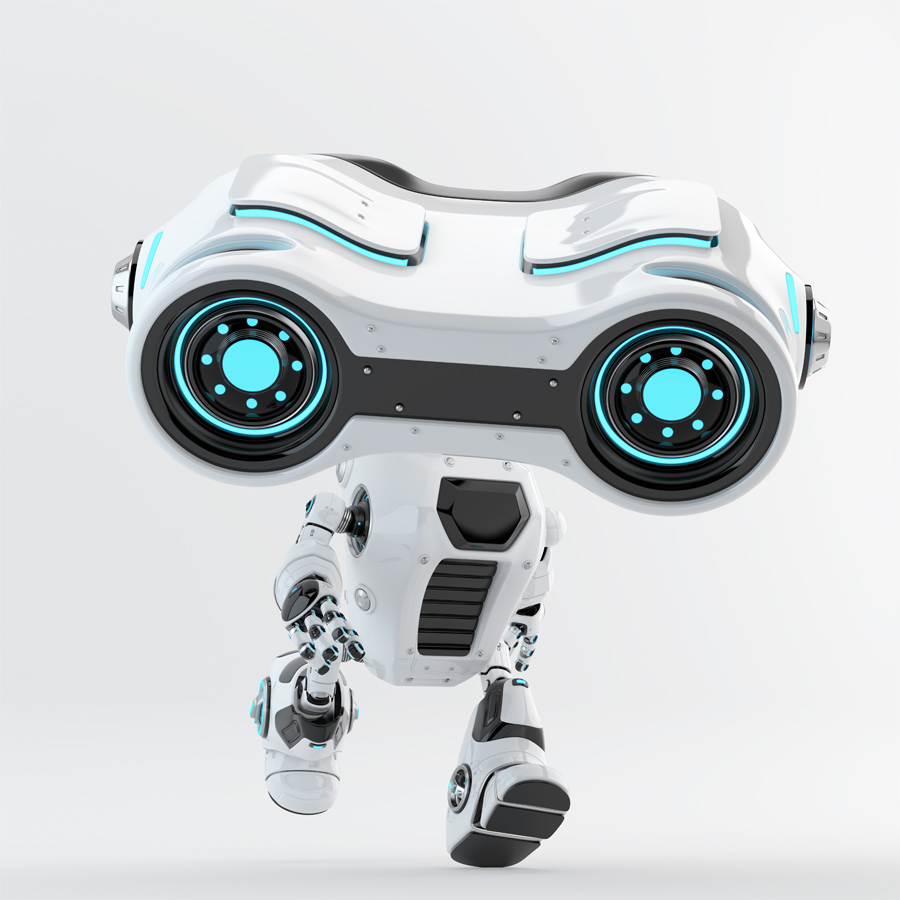
\includegraphics[scale=0.1]{images/look_robot.jpg}
\end{figure}
\end{frame}
\begin{frame}
\frametitle{Some solutions}
There are different solutions to approach this problem.\\
\begin{itemize}
\item<1 -> Supervised approach: threshold moving, sampling approach, anomaly detection, ...
\item<2 -> Unsupervised approach: isolation forest, ...
\end{itemize}
\end{frame}

\section{Brief mathematical recap on classification}
\begin{frame}
\frametitle{What is classification?}
\begin{itemize}
\item<1 -> Classification is a \textbf{supervised machine learning problem}.
\item<2 -> The mathematical model is in the general form of:
$$
p = f(X) + \varepsilon
$$
where $p$ is the \textbf{estimated probability} to belong to a certain class $Y$, $X$ the \textbf{input}, $\varepsilon$ an \textbf{error term}, $f$ is the \textbf{relationship} between the input and the output.
\end{itemize}
\end{frame}

\begin{frame}
\frametitle{Binary classification}
In binary classification:
\begin{itemize}
\item<1-> We select one of the two classes, that we call the "positive class" and $p$ is the probability to belong to this class
\item<2 -> $1-p$ is the probability for the other class, the "negative class".
\item<3 -> We classify using the probabilities according to a \textbf{threshold}.
\item<4 -> $\textbf{threshold} = 0.5$ in balanced classification.
\end{itemize}
\end{frame}

\begin{frame}
\frametitle{Metrics for binary classification}
\begin{itemize}
\item<1 -> We want to understand how many events are right predicted, how many mistakes have been done, and which ones.
\item<2 -> A classical tool is the \textbf{confusion matrix}.
\begin{figure}[ht]
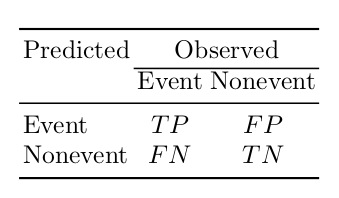
\includegraphics[scale=0.25]{images/confusionmatrix.png}
\caption{A general confusion matrix}
\end{figure}
\item<3 -> With this matrix we can create different metrics.
\end{itemize}
\end{frame}

\begin{frame}
\frametitle{Accuracy, Sensitivity, Specificity, Precision}
\begin{itemize}
\item<1 -> The \textbf{Accuracy rate} is defined as:
$$\dfrac{TP + TN}{TP + TN + FP + FN}.$$
\item<2 -> The \textbf{Sensitivity} (or \textbf{Recall}) is defined as: $$\dfrac{\mbox{TP}}{\mbox{TP + FN}}.$$
\item<3 -> The \textbf{Specificity} is defined as: $$\dfrac{\mbox{TN}}{\mbox{TN+FP}}.$$
\item<4 -> The \textbf{Precision} is defined as: $$\dfrac{\mbox{TP}}{TP + FP}.$$
\end{itemize}
\end{frame}
\section{The problem we will deal with}
\begin{frame}
\frametitle{Dataframe test}
\begin{itemize}
\item We will deal with the \textbf{TwoClassSim} dataset of the \textbf{caret package in R}.
\item We have two classes and we have chosen $99.52\%$ of the first class and $0.48\%$ of the second one.
\vspace{3mm}
\begin{figure}[ht]
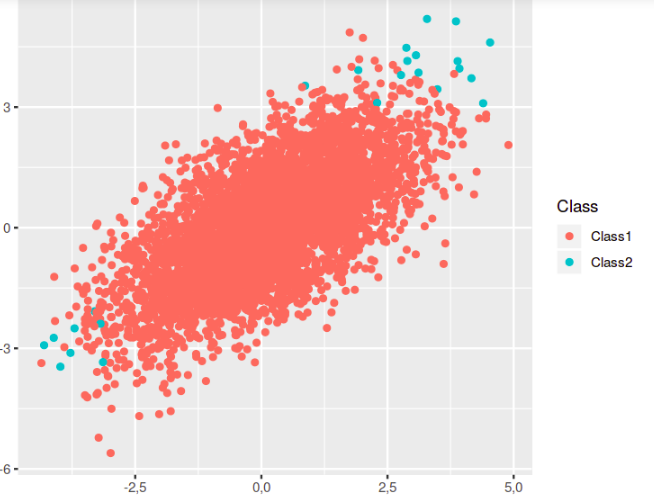
\includegraphics[scale=0.40]{images/twoclasssim.png}
\caption{A projection in 2D of the TwoClassSim dataset}
\end{figure}
\end{itemize}
\end{frame}

\begin{frame}
\frametitle{Using classical method for imbalanced problem}
\begin{itemize}

\item<1 -> We tried to use a classical approach to this problem optimizing the models w.r.t. the accuracy.
\item<2 -> We choose the less frequent class as positive
\begin{table}
\begin{tabular}{l | c | c | c | c }
Model & Accuracy & Sensitivity & Specificity  \\
\hline \hline
Random Forest  & 0.99 & 0.26 & 0.95 \\ 
Logistic Regression & 0.99 & 0.03 & 0.99\\
KNN & 0.99 & 0  & 1\\
\end{tabular}
\end{table}
\item<3 -> A naive model that predict all the sample as the negative one has an accuracy of $99\%$.
\item<4 -> It's clear that the models are focusing on the negative class.
\end{itemize}
\end{frame}

\begin{frame}
\frametitle{Pay attention}
\begin{center}
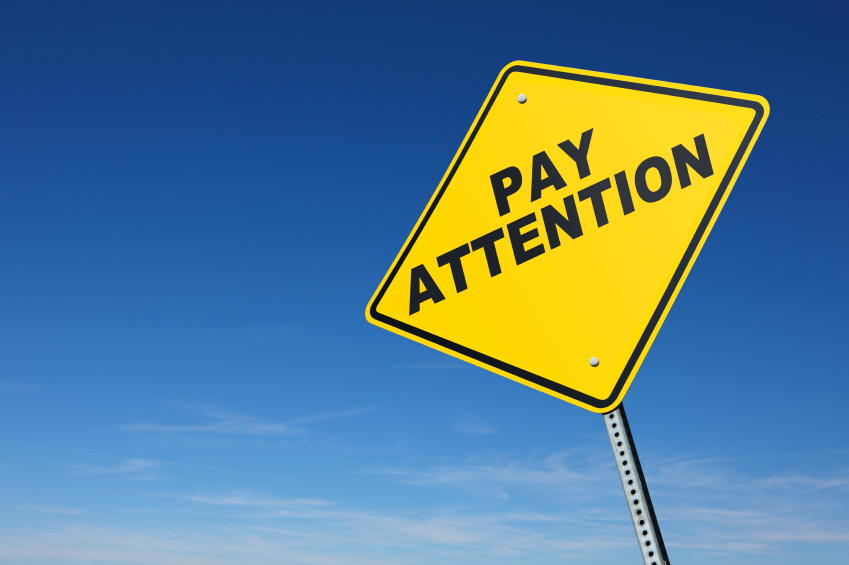
\includegraphics[scale=0.8]{images/payattention.jpeg}
\end{center}
\vspace{3mm}

\begin{itemize}
\item<1-> It's up to us to decide if we are more interested in a good positive class classification, in a negative one, or in a trade-off of them. 
\item<2-> \textbf{The techniques we have to use depends on the problem}.


\end{itemize}
\end{frame}
\section{Supervised method for imbalaced classification}
\begin{frame}
\frametitle{How can we approach the problem?}
To deal with the imbalance you can:
\begin{itemize}
\item<1 -> do nothing and cross your fingers.
\item<2 -> change the classification metric for optimizing.
\item<3 -> change the threshold cutoff to classify.
\item<4 -> use sampling methods.
\item<5 -> weigth the loss for a cost-sentivite training.
\end{itemize}
\end{frame}
\subsection{Classification metric method}
\begin{frame}
\frametitle{Changing the optimizing metric}
\begin{itemize}
\item<1 -> We can chose the best model through the different ones using the \textbf{accuracy metric}:
$$\dfrac{TP + TN}{TP + TN + FP + FN}.$$
\item<2 -> Problem: this metric is \textbf{too much oriented to the most frequent class} due to the difference of order of magnitude.
\item<3 -> Solution: we can optimize w.r.t. sensitivity, precision, AUC ROC curve, AUC precision-recall curve.
\end{itemize}
\end{frame}

\begin{frame}
\frametitle{ROC curve}
\begin{itemize}
\item<1 -> We have $1-\mbox{Specificity}$ on the $x-$ axis and $\mbox{Sensitivity}$ on the $y$-axis.
$$1-\mbox{Specificity}= 1 - \dfrac{\mbox{TN}}{\mbox{TN+FP}} = \dfrac{\mbox{FP}}{\mbox{TN+FP}}.$$
\item<2 -> The ROC curve is created changing the threshold for the model and predicting the associated label. After that we measure for each threshold/prediction step the Sensitivity and $1-\mbox{Specificity}$.
\vspace{2mm}
\begin{figure}[ht]
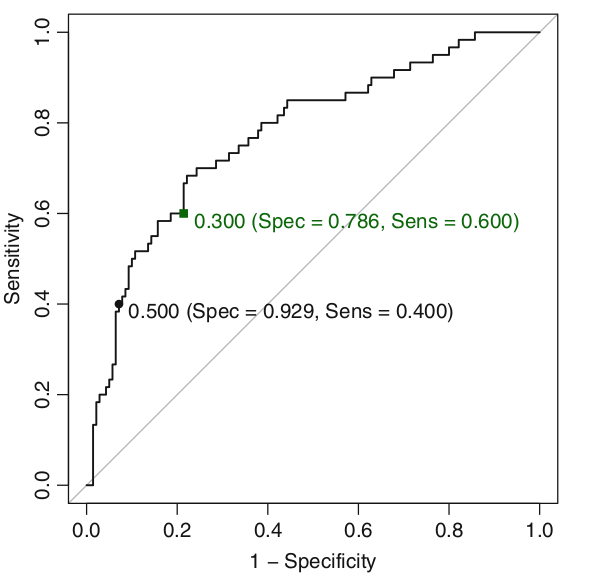
\includegraphics[scale=0.25]{images/ROC curve.png}
\caption{ROC curve of a classifier against random guess}
\end{figure}
\end{itemize}

\end{frame}

\begin{frame}
\frametitle{Some observations on the ROC curve}
\begin{itemize}
\item<1 -> The \textbf{bisector} is the ROC curve for the \textbf{random guessing}.
\item<2 -> A \textbf{perfect classifier} has a ROC curve of the type $\textbf{y=1}$. 
\item<3 -> We can use the \textbf{AUC of the ROC curve to select a model}.\\
$\Rightarrow$ threshold-insensitive.\\
$\Rightarrow$ insensitive to disparity in the class proportions (it's a function of sensitivity and specificity).\\
\end{itemize}
\end{frame}

\begin{frame}
\frametitle{Problems with AUC ROC curve}
Problems:
\begin{itemize}
\item<1 -> different \textbf{curves could cross}.
\item<2 -> the \textbf{threshold} can be an \textbf{important discriminating factor}.
\item<3 -> with very \textbf{imbalanced dataset is not reliable}.
\end{itemize}
\end{frame}
\begin{frame}
\frametitle{Example of ROC problem}
Let's see an example of the previous problem.\\
\begin{table}
\begin{tabular}{l | c | c | c | c }
Predicted | Reference & Negative & Positive \\
\hline \hline
Negative & 9.4e+04 & 10 \\ 
Positive &  4.4e+03 & 1.6e+02 \\
\end{tabular}
\end{table}
In this case we have:
\begin{itemize}
\item Sensitivity: 0.94
\item Specificity: 0.95
\item Precision: 0.035
\end{itemize}
\end{frame}


\begin{frame}
\frametitle{The ROC Problem}
\begin{itemize}
\item This is related to the fact that:
$$
FPR = 1 - \mbox{Specificity}= \dfrac{FP}{TN + FP}
$$
and $FP$ can be very different in order of magnitude with respect to $TN$. \\
$\Rightarrow$ we can have a $FP$ number high w.r.t. $TP$ but low w.r.t. $TN$. \\
$\Rightarrow$ the FPR becames always near to zero\\
$\Rightarrow$ the ROC curve seems similar to that one of the perfect classifier\\
\item we can have a very good recall and sensitivity and low precision.
\end{itemize}
\end{frame}

\begin{frame}
\frametitle{Precision-Recall Curve}
\begin{itemize}
\item<1-> According to the precision-recall trade-off we can also construct the precision-recall curve.
\vspace{2mm}
\begin{figure}[ht]
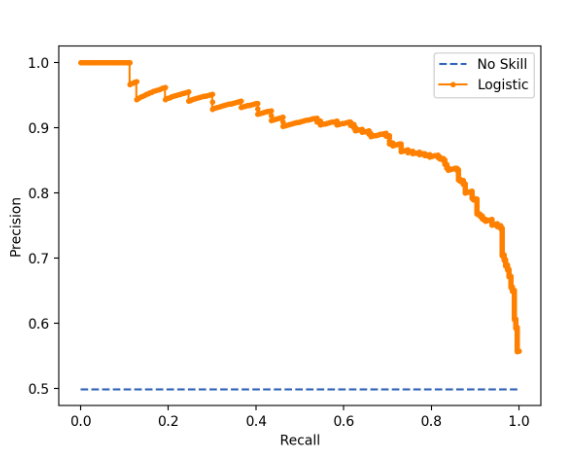
\includegraphics[scale=0.25]{images/precision-recall.png}
\caption{Precision-Recall curve}
\end{figure}
\item<2-> In this case too we can \textbf{select the best model} according to the \textbf{AUC of the precision-recall curve}.
\item<3 -> In a \textbf{very imbalanced dataset} (e.g 1:100) it's \textbf{better to use the precision-recall curve} because the ROC is optimistic.

\end{itemize}
\end{frame}



\begin{frame}
\frametitle{Numerical example}
Let's try to optimize a random forest w.r.t. the ROC:
\begin{table}
\begin{tabular}{l | c | c | c | c }
mtry & ROC & Sens & Spec & Accuracy \\
\hline \hline
2 & 0.95 & 0 & 1 & 0.995 \\ 
7 & 0.949 & 0 & 1 & 0.995 \\
13 & 0.97 & 0.13 & 0.999 & 0.995 \\
19 & 0.95 & 0.26 & 0.999 & 0.996 \\
25 & 0.944 & 0.23 & 0.999 & 0.995 \\
31 & 0.946 & 0.33 & 0.999 & 0.996 \\
37 & 0.947 & 0.35 & 0.999 & 0.995 \\
43 & 0.948 & 0.33 & 0.999 & 0.996 \\
49 & 0.925 & 0.38 & 0.998 & 0.996 \\
55 & 0.942 & 0.38 & 0.998 & 0.996 \\
\end{tabular}
\end{table}
\end{frame}

\subsection{Threshold selection method}
\begin{frame}
\frametitle{Threshold selection}
\begin{itemize}
\item<1 -> Having the probabilities we can \textbf{change the threshold to predict the associated labels}.
\item<2 -> Changing the threshold \textbf{we change sensitivity, specificitity, precision} and so on.
\item<3 -> We can use both the \textbf{ROC curve and the precision recall}.
\end{itemize}
\end{frame}

\begin{frame}
\frametitle{Select the threshold using a ROC curve}
\begin{itemize}
\item<1 -> Searching for the point nearest to the point with $100\%$ Sensitivity and $100\%$ Specificity (the top left corner) and chose the associated threshold.
\item<2 -> Searching the threshold that maximizes the \textbf{Youden's J index}:
$$
\textbf{J}(thr) = Sensitivity(thr) + Specificity(thr) - 1
$$
\item<3 ->  Searching the threshold that maximizes the \textbf{G-mean}:
$$
\textbf{G} = \sqrt{Sensitivity(thr)\cdot Specitificity(thr)}
$$
\begin{figure}[ht]
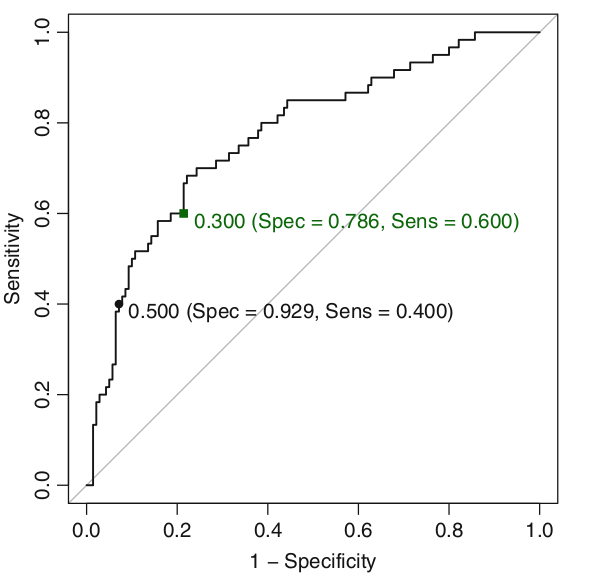
\includegraphics[scale=0.25]{images/ROC curve.png}
\end{figure}
\end{itemize}
\end{frame}

\begin{frame}
\frametitle{Numerical example}
We use a r.f. with $mtry = 13$ changing the threshold:
\begin{table}
\begin{tabular}{l | c | c | c | c }
Method & Threshold & Specificity & Sensitivity\\
\hline \hline
Default & 0.5  & 0.999 & 0.133 \\
Clos.topleft & 0.047 & 0.98 & 0.96 \\
Youden & 0.047 & 0.98 & 0.96 & \\

\end{tabular}
\end{table}
\end{frame}

\begin{frame}
\frametitle{Select the threshold using a precision-recall curve}
\begin{itemize}
\item<1-> Searching for the point nearest to the point with $100\%$ Precision and $100\%$ Recall (the top right corner) and chose the associated threshold.
\item<2->  Searching the threshold that maximizes the \textbf{F1-score}:
$$
\textbf{F}_1(thr) = \dfrac{2}{\dfrac{1}{\mbox{precision}(thr)}+ \dfrac{1}{\mbox{recall}(thr)}}
$$
\end{itemize}
\vspace{2mm}
\begin{figure}[ht]
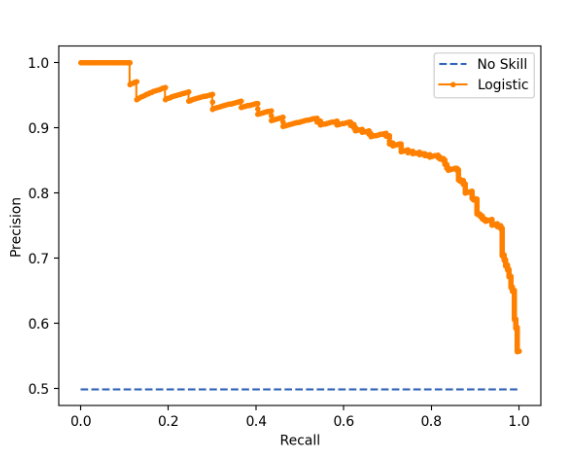
\includegraphics[scale=0.25]{images/precision-recall.png}
\caption{Precision-Recall curve}
\end{figure}
\end{frame}
\begin{frame}
\frametitle{How to select the threshold}
The threshold can be seen as a model parameter.\\
To select it we have to use:
\begin{itemize}
\item<1->  A \textbf{training set} for learning the different model and select the best one (using a threshold invariant metric)
\item<2->  An \textbf{evaluation set} to select the threshold.
\item<3->  A \textbf{test set} to have un unbiased estimation of the error.
\end{itemize}
\end{frame}
\begin{frame}
\frametitle{Pay attention}
\begin{center}
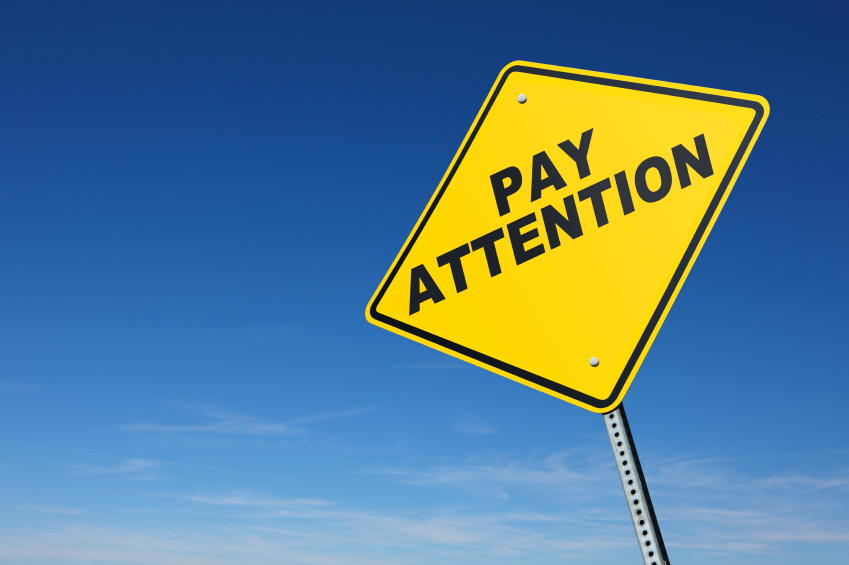
\includegraphics[scale=0.8]{images/payattention.jpeg}
\end{center}
\vspace{3mm}
\begin{itemize}
\item<1->  The core model doesn't change changing the threshold!
\item<2->  We only change the trade-off between particular type of errors.
\item<3->  In a confusion matrix we are moving up and down rows of the matrix and not moving from the off-diagonal to the diagonal.
\item<4->  We are not inducing further separation between the classes.

\end{itemize}
\end{frame}
\subsection{Sampling methods}
\begin{frame}
Different techniques to solve class imbalance:
\begin{itemize}
\item<1->  \textbf{Priori} technique: balance sampling more the less frequent class
\item<2->  \textbf{Post} technique: \begin{itemize}
\item<3->  \textbf{Up-sampling}
\item<4->  \textbf{Down-sampling}
\item<5->  \textbf{SMOTE}
\end{itemize}
\end{itemize}
\end{frame}

\begin{frame}
\frametitle{Priori sampling}
\begin{itemize}
\item<1->  We try to balance sampling the less frequent class at priori.
\item<2->  The training set $\Rightarrow$  can be balanced.
\item<3->  The test set $\Rightarrow$ must reflect the imbalance of the real data.
\item<4->  Sometimes is not possible to obtain more data.
\end{itemize}
\end{frame}

\begin{frame}
\frametitle{Post hoc sampling: Up-sampling}
\begin{itemize}
\item<1->  We \textbf{duplicate some of the data in the minority class}.

\item<2->  We use a sampling with replacement until we don't reach the same number of sample in each class.
\begin{figure}[ht]
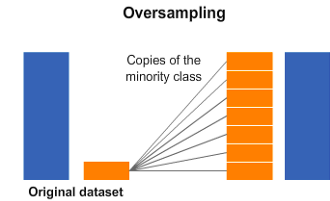
\includegraphics[scale=0.60]{images/Upsampling.png}
\caption{Upsampling Proceduce}
\end{figure}
\item<3->  We don't lose informations but we decrease the variability of our data.

\end{itemize}
\end{frame}


\begin{frame}
\frametitle{Post hoc sampling: Down-sampling}
\begin{itemize}
\item<1->  We \textbf{remove some of the data in the majority class}.
\item<2->  We remove at random until we don't reach the same number of sample in each class.
\begin{figure}[ht]
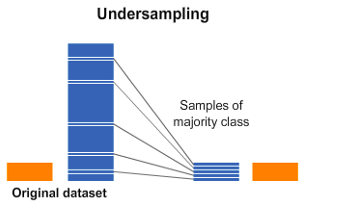
\includegraphics[scale=0.60]{images/Undersampling.png}
\caption{Downsampling Proceduce}
\end{figure}
\item<3->  We lose informations but we don't have big effect on the variability of our data.

\end{itemize}
\end{frame}

\begin{frame}
\frametitle{Post hoc sampling: SMOTE}
\begin{itemize}
\item<1->  Use both a down sampling and new up sampling.
\item<2->  The down-sampling is the previous one.
\item<3->  The up one is a Syntetic generation data using a KNN approach.
\item<4->  The generated sample is a random combination of randomly selected data points.
\end{itemize}
\end{frame}

\begin{frame}
\frametitle{SMOTE algorithm: downsampling phase}
\begin{itemize}
\item<1->  Randomly remove sample from majority class population until minority class becomes some specified percentage of minority class. 
\item<2->  e.g.: 
\begin{itemize}
\item majority class: 200 sample
\item minority class: 50 sample
\item Percentage we down: $200\%$.
\end{itemize}
$\Rightarrow$ majority class: 25 sample.
\item<3->  Percentage of downsample of majority class $\Rightarrow$ Parameter to tune.
\end{itemize}
\end{frame}

\begin{frame}
\frametitle{SMOTE algorithm: syntetic generation}
\begin{itemize}
\item<1->  Select a parameter $k$ to define the \textbf{number of neighbors} to take.
\item<2->  Select a \textbf{percentage of the minority class} to generate.
\item<3->  \textbf{For each point of the minority class} take the $k$ neighbors and according to the percentage to generate \textbf{take random neighbors from the $k$ ones}
\item<4->  For each point take a random \textbf{convex combination} between the point and each neighbors.
\item<5->  The point obtained with the combination is the \textbf{new sintetic generated one}.
\end{itemize}
\end{frame}

\begin{frame}
\frametitle{When do we have to sample?}
Different moments when we can use sampling methods:
\begin{itemize}
\item<1->  Before the cross validation\\
$\Rightarrow$ the dev error is biased.\\
$ \Rightarrow$ less computational cost.
\item<2->  During the cross validation\\
$\Rightarrow$ the dev error is not biased.\\
$\Rightarrow$ more computational cost.
\end{itemize}
\end{frame}

\begin{frame}
\frametitle{Numerical example}
We tried to compare the three sampling methods with a logistic regression:
\begin{table}
\begin{tabular}{l | c | c | c | c }
Method & ROC  & Sensitivity & Specificity & Accuracy\\
\hline \hline
No sampling & 0,759 & 0,05 & 0,998 & 0,99 \\
Up & 0,62 & 0,65 & 0,56 & 0,56 \\
Down & 0,62 & 0,65 & 0,56 & 0,56 \\
SMOTE & 0,63 & 0,53 & 0,757 & 0,757\\ 
\end{tabular}
\end{table}
\end{frame}

\begin{frame}
\frametitle{Pay attention}
\begin{center}
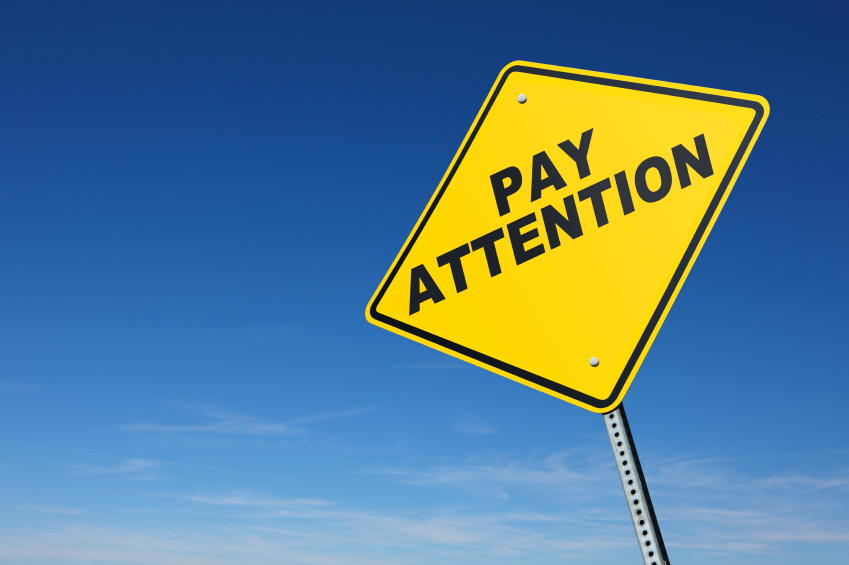
\includegraphics[scale=0.8]{images/payattention.jpeg}
\end{center}
\vspace{3mm}

\begin{itemize}
\item<1 -> We have to apply the \textbf{post sampling only on the training set} to better learn.
\item<2 -> The \textbf{test set} must follow the \textbf{original distribution}.
\item<3 -> Using a sampling method on the test set will result in a \textbf{biased error}.
\end{itemize}

\end{frame}
\subsection{Cost-sensitive training}
\begin{frame}
\frametitle{Introducing a new loss}
\begin{itemize}
\item<1->  We can optimize a modified loss function instead of the classical one.
\item<2->  The new loss weights the two classes differently.
\item<3->  This affect the parameters and can have significant improvements.
\end{itemize}
\end{frame}

\begin{frame}
\frametitle{Some examples}
\begin{itemize}
\item<1->  Loss for logistic regression:
$$
\textit{L} = \sum_{i = 1}^{n}w_i\cdot y_i \cdot \mbox{log}\hat{y}_i
$$
\item<2->  Gini index for a tree:
$$
Gini = C(1|2) p_1 (1-p_1) + C(2|1) p_2 (1-p_2)
$$
where $C(1|2)$ and $C(2|1)$ are the weights of missclassification.
\item<3->  We cannot have probabilities. They makes no sense. We cannot optimize w.r.t. ROC
\end{itemize}
\end{frame}

\begin{frame}
\frametitle{A numerical example}
We use a weighted loss for our example:
\begin{figure}[ht]
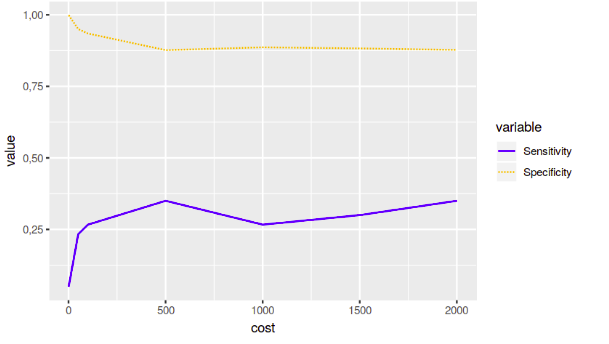
\includegraphics[scale=0.50]{images/weightplot.png}
\caption{Sensitivity and Specificity against the weight}
\end{figure}

\end{frame}
\section{The Bibliography}
\begin{thebibliography}{9}
\bibitem{apm}
Max Kuhn, Kjell Johnson: \textit{Applied Predictive Modeling}. Springer, 2016.

\bibitem{lfid}
Tom Fawcett: \textit{Learning from Imbalanced dataset}. \href{https://www.svds.com/learning-imbalanced-classes/}{Link to the article}.
\bibitem{hci}Wicked Good Data - r: \textit{Handling class imbalance with R and Caret - An introduction}. \href{https://www.r-bloggers.com/2016/12/handling-class-imbalance-with-r-and-caret-an-introduction/}{Link to the article}

\bibitem{gitic}Jason Brownlee: \textit{A Gentle Introduction to Imbalanced Classification}. \href{https://machinelearningmastery.com/what-is-imbalanced-classification/}{Link to the article}.
\bibitem{kn} LCT14558: \textit{Imbalanced data and why you should NOT use ROC curve} \href{https://www.kaggle.com/lct14558/imbalanced-data-why-you-should-not-use-roc-curve}{Link to the notebook}.
\bibitem{gittmfic}Jason Brownlee: \textit{A Gentle Introduction to Threshold-Moving for Imbalanced Classification}. \href{https://machinelearningmastery.com/threshold-moving-for-imbalanced-classification/}{Link to the article}.
\bibitem{smoteoriginal}
Nitesh V. Chawla, Kevin W. Bowyer, Lawrence O. Hall, W. Philip Kegelmeyer: \textit{SMOTE: Synthetic Minority Over-sampling Technique}. Journal of Artificial Intelligence Research 16 (2002) 321–357
\bibitem{sficwp} Jason Brownlee: \textit{SMOTE for Imbalanced Classification with Python} \href{https://machinelearningmastery.com/smote-oversampling-for-imbalanced-classification/}{Link to the article}.



\end{thebibliography}
\section*{Greetings}
\begin{frame}
\begin{figure}[ht]
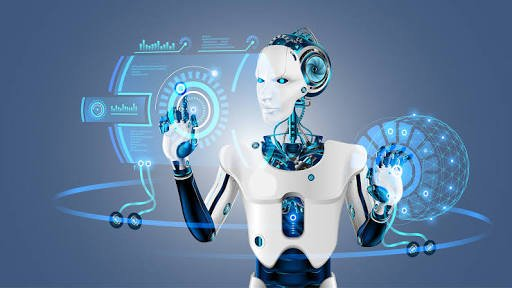
\includegraphics[scale=0.25]{images/thankyou.jpeg}
\end{figure}
  \centering \Huge
  \emph{\textbf{Thank you for your attention!!}}
\end{frame}
\end{document}